%Tipo de documento y otras especificaciones
\documentclass[12pt,letterpaper]{article}

% Para escribir tildes y eñes
\usepackage[utf8]{inputenc}  
\usepackage{listings}
% Para que los títulos de figuras, tablas y otros estén en español
\usepackage[spanish]{babel} 

% Cambiar nombre a tablas
\addto\captionsspanish{\renewcommand{\tablename}{Tabla}}          
% Cambiar nombre a lista de tablas
\addto\captionsspanish{\renewcommand{\listtablename}{Índice de tablas}}  

% Tamaño del área de escritura de la página
\usepackage{geometry}
\geometry{left=18mm,right=18mm,top=21mm,bottom=21mm} 
\usepackage{ucs}

% Los paquetes ams son desarrollados por la American Mathematical Society y mejoran la escritura de fórmulas y símbolos matemáticos.
\usepackage{amsmath}      
\usepackage{amsfonts}  \usepackage{listings}
\usepackage{amssymb}

% Para insertar gráficas
\usepackage{graphicx}

% Para colocar varias figuras
\usepackage[lofdepth,lotdepth]{subfig}

% Para la presentación correcta de unidades
\usepackage{unitsdef}

% Redimensionamiento del espacio entre magnitud y unidad
\renewcommand{\unitvaluesep}{\hspace*{4pt}}  

% Para insertar hipervínculos y marcadores
\usepackage[colorlinks=true,urlcolor=blue,linkcolor=black,citecolor=green]{hyperref}

% Para ubicar las tablas y figuras justo después del texto
\usepackage{float}
\usepackage{listings}
% Para hacer tablas más estilizadas
\usepackage{booktabs}  
\batchmode
\bibliographystyle{plain}
\pagestyle{plain}

% Para importar paginas PDF
\usepackage{pdfpages}

\pagenumbering{arabic}
\usepackage{lastpage}
\graphicspath{{./Figuras/}}

% Para manejar los encabezados y pies de página
\usepackage{fancyhdr}  
%verilog
\usepackage{xcolor}
\usepackage{listings}
\definecolor{vgreen}{RGB}{104,180,104}
\definecolor{vblue}{RGB}{49,49,255}
\definecolor{vorange}{RGB}{255,143,102}
\lstdefinestyle{verilog-style}
{
    language=Verilog,
    basicstyle=\small\ttfamily,
    keywordstyle=\color{vblue},
    identifierstyle=\color{black},
    commentstyle=\color{vgreen},
    tabsize=8,
    moredelim=*[s][\colorIndex]{[}{]},
    literate=*{:}{:}1
}
\makeatletter
\newcommand*\@lbracket{[}
\newcommand*\@rbracket{]}
\newcommand*\@colon{:}
\newcommand*\colorIndex{%
    \edef\@temp{\the\lst@token}%
    \ifx\@temp\@lbracket \color{black}%
    \else\ifx\@temp\@rbracket \color{black}%
    \else\ifx\@temp\@colon \color{black}%
    \else \color{vorange}%
    \fi\fi\fi
}
\makeatother

\usepackage{trace}

% Contenido de los encabezados y pies de pagina
\pagestyle{fancy}    
\lhead{IE-1014}
\chead{}
\rhead{ 
}
\lfoot{Escuela de Ingeniería Eléctrica}
\cfoot{\thepage\ de \pageref{LastPage}}
\rfoot{Universidad de Costa Rica}

\author{ Luis Benavides - B40953 \\{\small \bigskip \bigskip}}
\title{{ \begin{Huge}Universidad de Costa Rica \\\bigskip \bigskip \bigskip \bigskip \bigskip \end{Huge} IE-1014: Reconocimiento de Patrones  \\\bigskip \bigskip \bigskip \bigskip  }    
Tarea 1 \\\bigskip \bigskip \bigskip \bigskip \bigskip \bigskip \bigskip \bigskip \bigskip \bigskip Rer. Nat. Francisco Siles Canales \bigskip \bigskip \bigskip \bigskip \bigskip}

%\date{}      

\let\OLDthebibliography=\thebibliography
\def\thebibliography#1{\OLDthebibliography{#1}%
\addcontentsline{toc}{section}{\refname}}

\makeatletter
\renewcommand\@biblabel[1]{#1. \ }
\makeatother

% Inicio del documento
%%%%%%%%%%%%%%%%
\begin{document}  
%%%%%%%%%%%%%%%%



\begin{titlepage}

\newcommand{\HRule}{\rule{\linewidth}{0.5mm}} % Defines a new command for the horizontal lines, change thickness here

\center % Center everything on the page
 
%----------------------------------------------------------------------------------------
%  HEADING SECTIONS
%----------------------------------------------------------------------------------------
\textsc{\LARGE UNIVERSIDAD DE COSTA RICA}\\[1.5cm] % Name of your university/college
\textsc{\Large Escuela de Ingeniería Eléctrica}\\[0.5cm] % Major heading such as course name
\textsc{\large IE-1014: Introducción al Reconocimiento de Patrones }\\[0.5cm] % Minor heading such as course title

%----------------------------------------------------------------------------------------
%  TITLE SECTION
%----------------------------------------------------------------------------------------
\bigskip
\bigskip
\bigskip
\bigskip

\HRule \\[0.4cm]
{ \huge \bfseries Clasificacion  KNN con C++ }\\[0.4cm]
%\LARGE  %escribir aqui subtítulo 
 % Title of your document
\HRule \\[1.5cm]


 
%----------------------------------------------------------------------------------------
%  AUTHOR SECTION
%----------------------------------------------------------------------------------------

\begin{center} \large
Prof. Rer. Nat. Francisco Siles Canales\\ \bigskip
\bigskip
Grupo 1 \\ \bigskip
\bigskip
\bigskip
Estudiante:\\ 
 Luis Benavides Arias - B40953

 
% Your name
\end{center}
\bigskip
\bigskip
\bigskip
\bigskip
\bigskip
\bigskip
\bigskip
\bigskip
\bigskip
\bigskip
\bigskip
\bigskip
\bigskip
\bigskip
\bigskip
\normalsize \today \vspace*{5\baselineskip}

% If you don't want a supervisor, uncomment the two lines below and remove the section above
%\Large \emph{Author:}\\
%John \textsc{Smith}\\[3cm] % Your name

%----------------------------------------------------------------------------------------
%  DATE SECTION
%----------------------------------------------------------------------------------------



%----------------------------------------------------------------------------------------
%  LOGO SECTION
%----------------------------------------------------------------------------------------


 
%----------------------------------------------------------------------------------------

\vfill % Fill the rest of the page with whitespace

\end{titlepage}

\newpage

%%%%%%%%%%%%%%%%%%%%%%%%%%
\section*{Resumen}

Modifique el código de kMeans para poder realizar una clasificación kNN. Pruebe su código con los datos de iris y compare con los resultados obtenidos con weka.

Utilice otro conjunto distinto de datos de entrada anotados y obtenga una clasificación utilizando el código desarrollado. Comente los resultados obtenidos.

\section{Introducción}

El algoritmo de los k vecinos mas cercanos diseñado en C++, se basa en metricas euclideanas, con las cuales se procede a calcular asignaciones de clasificacion de datos desconocidos a datos dentro del conjunto de datos en cuestion, y determinar, segun la cantidad de vecinos mas cercanos, la variabilidad que tiene el conjunto de datos con respecto a sus elementos cercanos entre si.


\section{Resultados}

\subsection{Resultados Mediante Weka}

Utilizando el Dataset iris.arff, con el que hemos trabajado todo este tiempo, se hace uso del algoritmo Lazy IBk de Weka, para determinar cuanto varia el codigo creado a los resultados que se obtienen con weka. Se obtienen los siguientes resultados:


Para el caso de k=1:
\begin{lstlisting}
=== Run information ===

Scheme:weka.classifiers.lazy.IBk -K 1 -W 0 -A "weka.core.neighboursearch.LinearNNSearch -A \"weka.core.EuclideanDistance -R first-last\""
Relation:     iris
Instances:    149
Attributes:   5
              5.1
              3.5
              1.4
              0.2
              Iris-setosa
Test mode:10-fold cross-validation

=== Classifier model (full training set) ===

IB1 instance-based classifier
using 1 nearest neighbour(s) for classification


Time taken to build model: 0 seconds

=== Stratified cross-validation ===
=== Summary ===

Correctly Classified Instances       ||  142   ||            95.302  %
Incorrectly Classified Instances      ||   7    ||           4.698  %
Kappa statistic                          0.9295
Mean absolute error                      0.0402
Root mean squared error                  0.1753
Relative absolute error                  9.0424 %
Root relative squared error             37.1909 %
Total Number of Instances              149     

=== Detailed Accuracy By Class ===

               TP Rate   FP Rate   Precision   Recall  F-Measure   ROC Area  Class
                 1         0          1         1         1          1        Iris-setosa
                 0.94      0.04       0.922     0.94      0.931      0.95     Iris-versicolor
                 0.92      0.03       0.939     0.92      0.929      0.942    Iris-virginica
Weighted Avg.    0.953     0.024      0.953     0.953     0.953      0.964

=== Confusion Matrix ===

  a  b  c   <-- classified as
 49  0  0 |  a = Iris-setosa
  0 47  3 |  b = Iris-versicolor
  0  4 46 |  c = Iris-virginica
\end{lstlisting}

Para el codigo creado en c++, ejecutandose para k=1, se obtiene el siguiente resultado:

\begin{figure}[H]
    \centering
    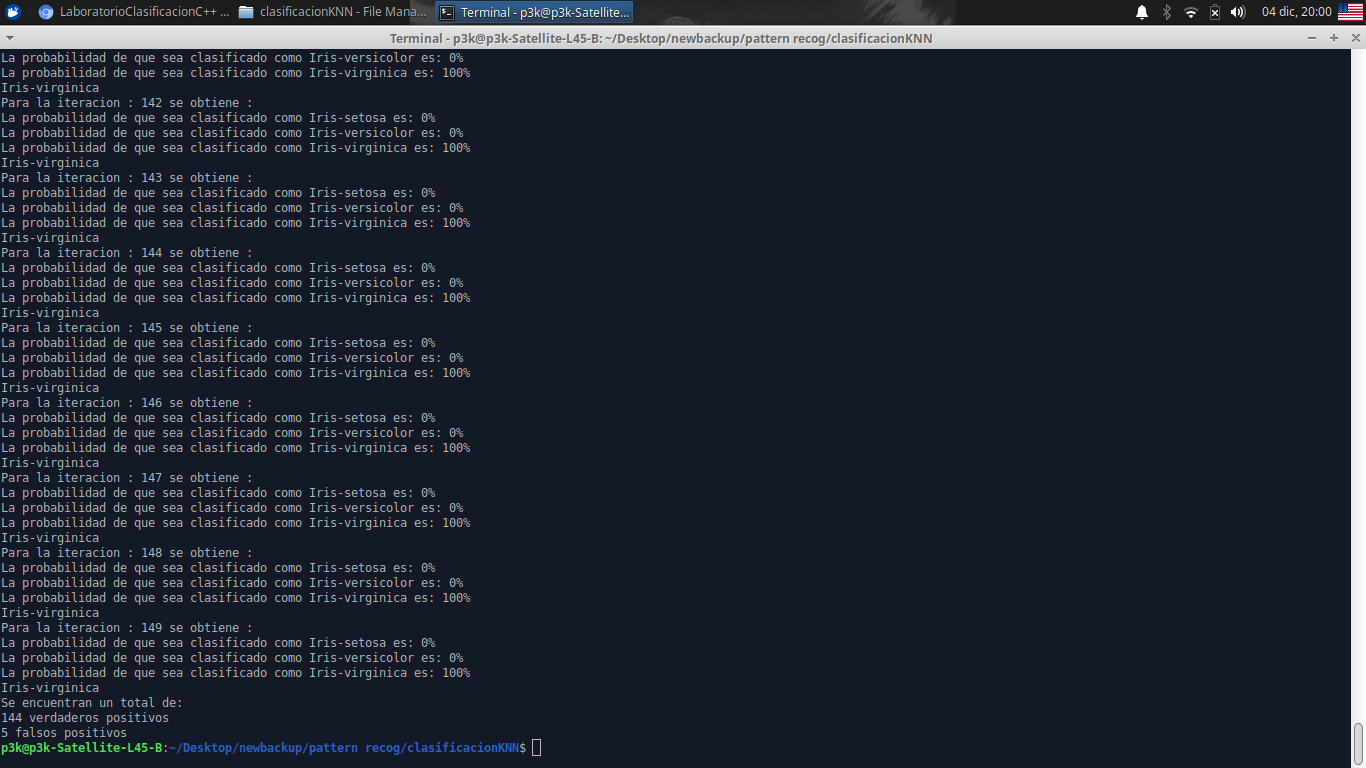
\includegraphics[width=0.8\textwidth]{knnc++1.jpg}
    \caption{Resultado del codigo en c++, para k=1}
    \label{fig:1}
\end{figure}

Para el caso k=2;

\begin{lstlisting}
=== Run information ===

Scheme:weka.classifiers.lazy.IBk -K 2 -W 0 -A "weka.core.neighboursearch.LinearNNSearch -A \"weka.core.EuclideanDistance -R first-last\""
Relation:     iris
Instances:    149
Attributes:   5
              5.1
              3.5
              1.4
              0.2
              Iris-setosa
Test mode:10-fold cross-validation

=== Classifier model (full training set) ===

IB1 instance-based classifier
using 2 nearest neighbour(s) for classification


Time taken to build model: 0 seconds

=== Stratified cross-validation ===
=== Summary ===

Correctly Classified Instances         143               95.9732 %
Incorrectly Classified Instances         6                4.0268 %
Kappa statistic                          0.9396
Mean absolute error                      0.038 
Root mean squared error                  0.1666
Relative absolute error                  8.5608 %
Root relative squared error             35.3323 %
Total Number of Instances              149     

=== Detailed Accuracy By Class ===

               TP Rate   FP Rate   Precision   Recall  F-Measure   ROC Area  Class
                 1         0          1         1         1          1        Iris-setosa
                 0.96      0.04       0.923     0.96      0.941      0.962    Iris-versicolor
                 0.92      0.02       0.958     0.92      0.939      0.954    Iris-virginica
Weighted Avg.    0.96      0.02       0.96      0.96      0.96       0.972

=== Confusion Matrix ===

  a  b  c   <-- classified as
 49  0  0 |  a = Iris-setosa
  0 48  2 |  b = Iris-versicolor
  0  4 46 |  c = Iris-virginica
\end{lstlisting}

Para k=2, se obtienen los siguientes resultados:

\begin{figure}[H]
    \centering
    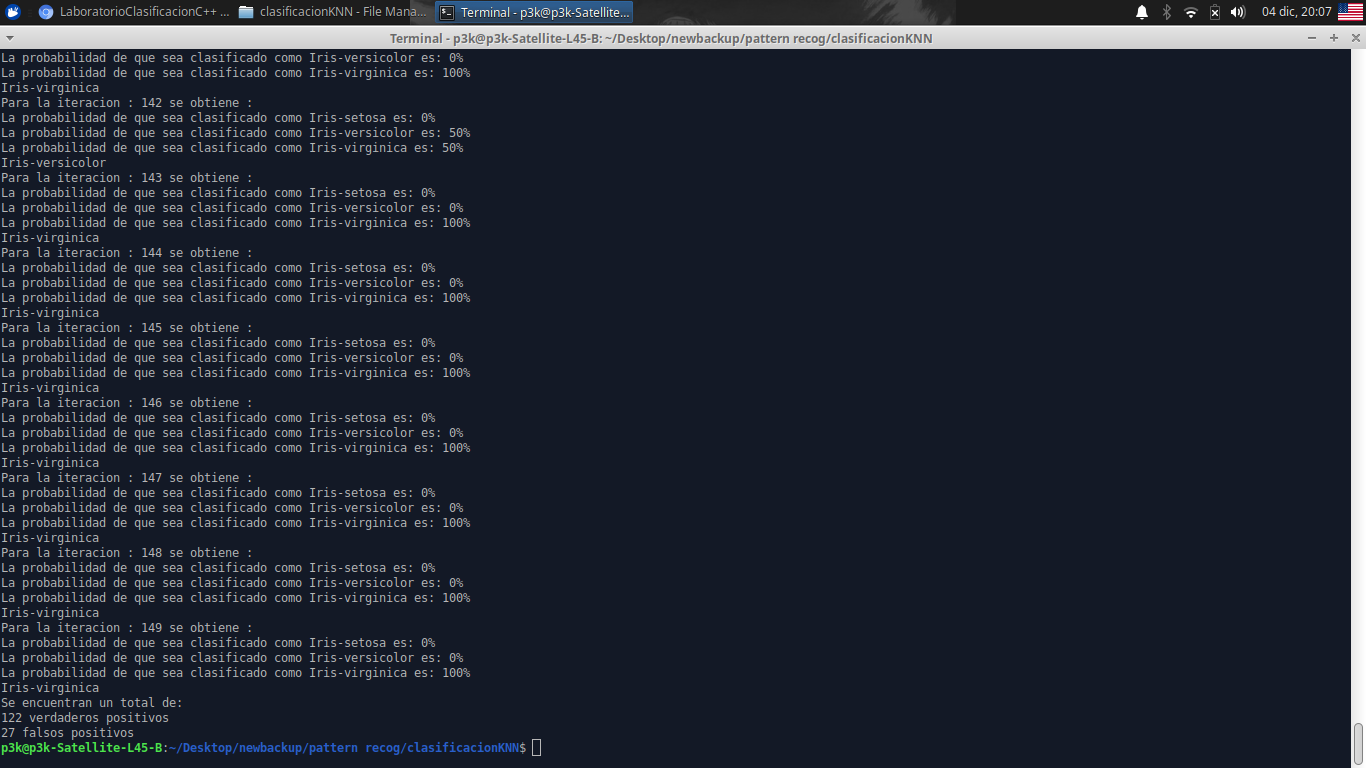
\includegraphics[width=0.8\textwidth]{knnc++2.jpg}
    \caption{Resultado codigo c++, para k=2}
    \label{fig:2}
\end{figure}

Para el caso k=3:

\begin{lstlisting}
=== Run information ===

Scheme:weka.classifiers.lazy.IBk -K 3 -W 0 -A "weka.core.neighboursearch.LinearNNSearch -A \"weka.core.EuclideanDistance -R first-last\""
Relation:     iris
Instances:    149
Attributes:   5
              5.1
              3.5
              1.4
              0.2
              Iris-setosa
Test mode:10-fold cross-validation

=== Classifier model (full training set) ===

IB1 instance-based classifier
using 3 nearest neighbour(s) for classification


Time taken to build model: 0 seconds

=== Stratified cross-validation ===
=== Summary ===

Correctly Classified Instances         143               95.9732 %
Incorrectly Classified Instances         6                4.0268 %
Kappa statistic                          0.9396
Mean absolute error                      0.0403
Root mean squared error                  0.1679
Relative absolute error                  9.0625 %
Root relative squared error             35.6255 %
Total Number of Instances              149     

=== Detailed Accuracy By Class ===

               TP Rate   FP Rate   Precision   Recall  F-Measure   ROC Area  Class
                 1         0          1         1         1          1        Iris-setosa
                 0.96      0.04       0.923     0.96      0.941      0.962    Iris-versicolor
                 0.92      0.02       0.958     0.92      0.939      0.953    Iris-virginica
Weighted Avg.    0.96      0.02       0.96      0.96      0.96       0.971

=== Confusion Matrix ===

  a  b  c   <-- classified as
 49  0  0 |  a = Iris-setosa
  0 48  2 |  b = Iris-versicolor
  0  4 46 |  c = Iris-virginica
\end{lstlisting}

\begin{figure}[H]
    \centering
    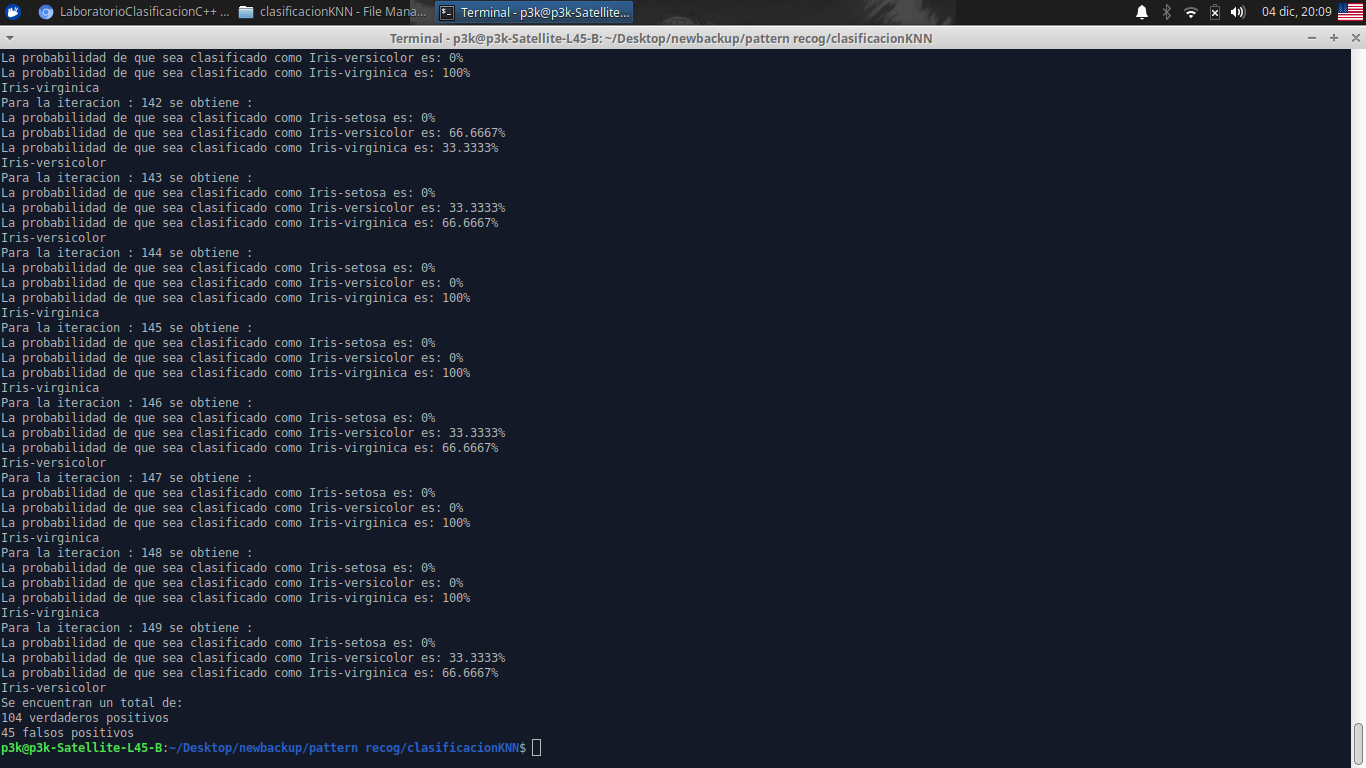
\includegraphics[width=0.8\textwidth]{knnc++3.jpg}
    \caption{Resultado codigo en c++, para k=3}
    \label{fig:3}
\end{figure}

Ahora para k=5:

\begin{lstlisting}
=== Run information ===

Scheme:weka.classifiers.lazy.IBk -K 5 -W 0 -A "weka.core.neighboursearch.LinearNNSearch -A \"weka.core.EuclideanDistance -R first-last\""
Relation:     iris
Instances:    149
Attributes:   5
              5.1
              3.5
              1.4
              0.2
              Iris-setosa
Test mode:evaluate on training data

=== Classifier model (full training set) ===

IB1 instance-based classifier
using 5 nearest neighbour(s) for classification


Time taken to build model: 0 seconds

=== Evaluation on training set ===
=== Summary ===

Correctly Classified Instances         143               95.9732 %
Incorrectly Classified Instances         6                4.0268 %
Kappa statistic                          0.9396
Mean absolute error                      0.033 
Root mean squared error                  0.1304
Relative absolute error                  7.4174 %
Root relative squared error             27.655  %
Total Number of Instances              149     

=== Detailed Accuracy By Class ===

               TP Rate   FP Rate   Precision   Recall  F-Measure   ROC Area  Class
                 1         0          1         1         1          1        Iris-setosa
                 0.96      0.04       0.923     0.96      0.941      0.996    Iris-versicolor
                 0.92      0.02       0.958     0.92      0.939      0.996    Iris-virginica
Weighted Avg.    0.96      0.02       0.96      0.96      0.96       0.997

=== Confusion Matrix ===

  a  b  c   <-- classified as
 49  0  0 |  a = Iris-setosa
  0 48  2 |  b = Iris-versicolor
  0  4 46 |  c = Iris-virginica
\end{lstlisting}

\begin{figure}[H]
    \centering
    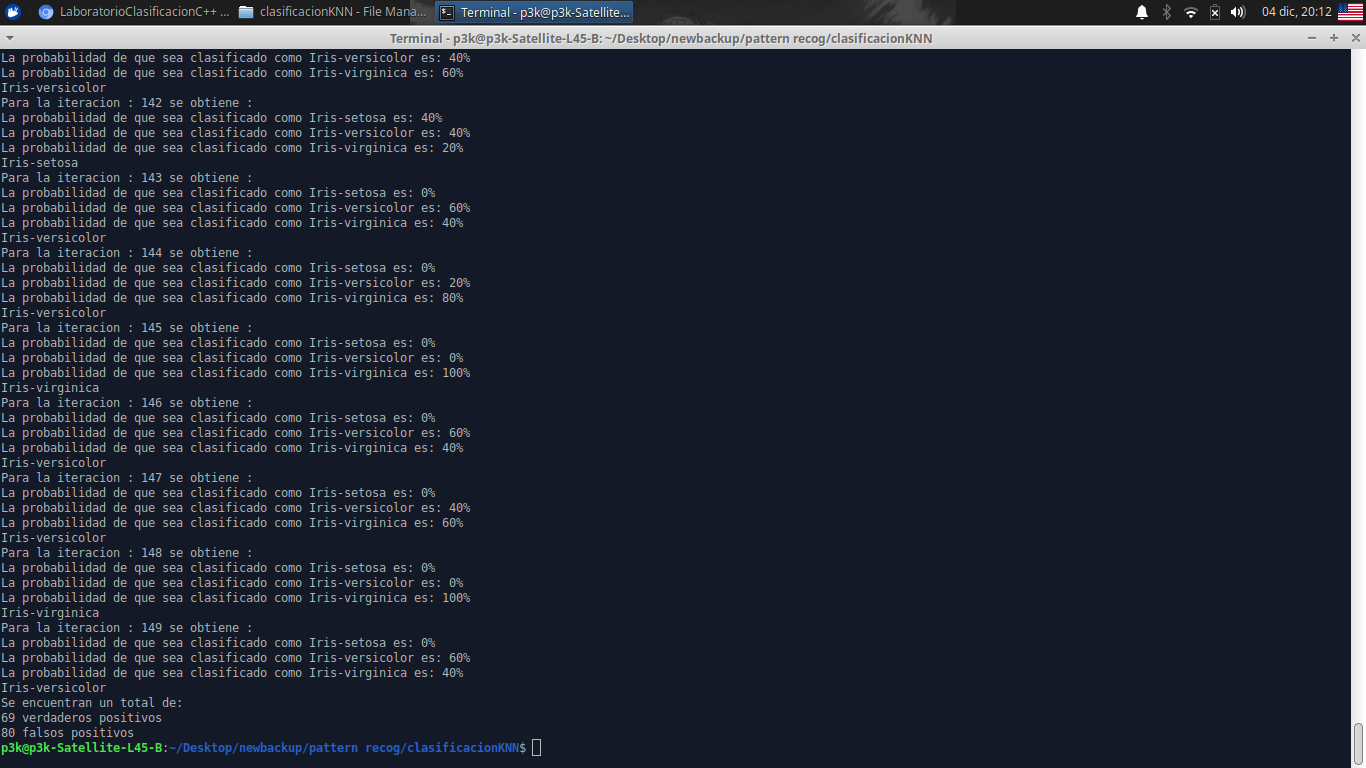
\includegraphics[width=0.8\textwidth]{knnc++5.jpg}
    \caption{Resultado codigo en c++, para k=5}
    \label{fig:5}
\end{figure}

Para k=10:

\begin{lstlisting}
=== Run information ===

Scheme:weka.classifiers.lazy.IBk -K 10 -W 0 -A "weka.core.neighboursearch.LinearNNSearch -A \"weka.core.EuclideanDistance -R first-last\""
Relation:     iris
Instances:    149
Attributes:   5
              5.1
              3.5
              1.4
              0.2
              Iris-setosa
Test mode:evaluate on training data

=== Classifier model (full training set) ===

IB1 instance-based classifier
using 10 nearest neighbour(s) for classification


Time taken to build model: 0 seconds

=== Evaluation on training set ===
=== Summary ===

Correctly Classified Instances         144               96.6443 %
Incorrectly Classified Instances         5                3.3557 %
Kappa statistic                          0.9497
Mean absolute error                      0.0346
Root mean squared error                  0.1128
Relative absolute error                  7.7813 %
Root relative squared error             23.9193 %
Total Number of Instances              149     

=== Detailed Accuracy By Class ===

               TP Rate   FP Rate   Precision   Recall  F-Measure   ROC Area  Class
                 1         0          1         1         1          1        Iris-setosa
                 0.98      0.04       0.925     0.98      0.951      0.998    Iris-versicolor
                 0.92      0.01       0.979     0.92      0.948      0.998    Iris-virginica
Weighted Avg.    0.966     0.017      0.968     0.966     0.966      0.999

=== Confusion Matrix ===

  a  b  c   <-- classified as
 49  0  0 |  a = Iris-setosa
  0 49  1 |  b = Iris-versicolor
  0  4 46 |  c = Iris-virginica
\end{lstlisting}
\begin{figure}[H]
    \centering
    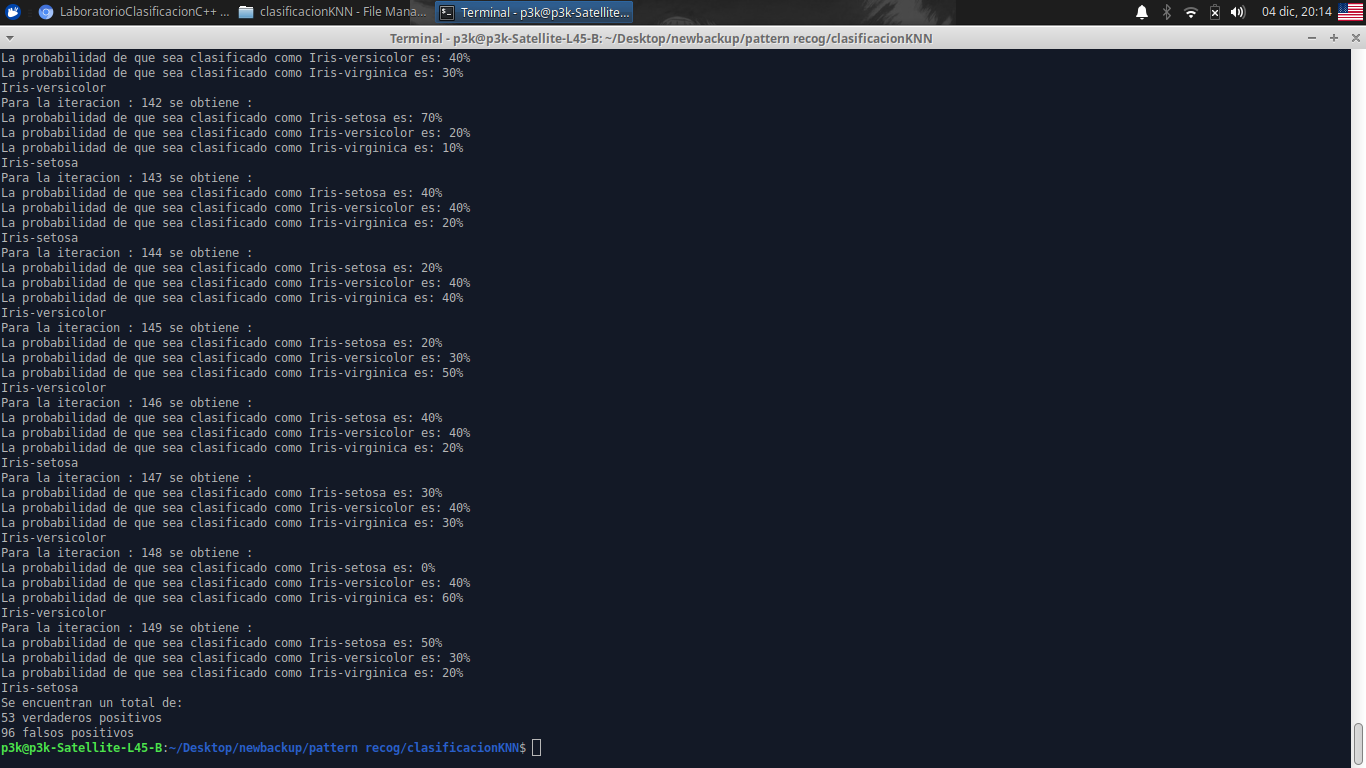
\includegraphics[width=0.8\textwidth]{knnc++10.jpg}
    \caption{Resultado codigo en c++, para k=10}
    \label{fig:10}
\end{figure}



\section{Analisis de datos y comparacion}

Se puede observar que mediante el algoritmo de Weka, el comportamiento al aumentar los k valores mas cercanos, se mantiene casi constante para datos menores a 5, y para valores mayores su precision disminuye.

Sin embargo, la variabilidad de los datos no se presenta gravemente a travez del set de datos, utilizando el codigo creado. Entre las razones pueden estar, el mal planteamiento del algoritmo, en cuanto a la precision al ordenar los datos, la forma en que se clasifican las clases por iteracion, o los casos que determinan la cantidad de clases por iteracion, entre los valores mas cercanos. Sin embargo, para valores pequeños de k, se obtienen buenas respuestas, muy similares a las de weka.

Se puede observar mediante weka, que las clasificaciones erroneas se presentan entre mayor sea el numero de vecinos cercanos contemplados por el algoritmo.

Ademas, el algoritmo elaborado no presenta analisis de la probabilidad media de error, la cual presenta \cite{duda} en su libro Pattern Clasification, esto debido a una ventana temporal de trabajo limitada, que apesar de que fue extendida mediante un tiempo de gracia, no fue suficiente para integrar estos analisis.


\section{Conclusiones}

Se concluye que construir un algoritmo para ejecutar un metodo de clasificacion, no es una labor trivial, y que conlleva tiempo depurarlo de forma eficiente. Tambien, por limitaciones de tiempo, y conocimiento, se presentan errores dentro del algoritmo, por el desconocimiento del lenguaje C++.

Se concluye que el algoritmo creado, para k pequeños, presenta buenas metricas, pero no se logran ejecutar las metricas de validacion como Precision, Recall y F-Measure, ni ROC Area.


\begin{thebibliography}{}
%\bibitem{eie} Escuela de Ingeniería Eléctrica. Laboratorios de investigación https://eie.ucr.ac.cr/laboratorios/?tipo=Investigaci\%C3\%B3n

%\bibitem{PRIS-Lab} PRIS-Seminar 2018, recuperado de \url{https://www.youtube.com/channel/UCKHRBb_Wxuv1f_7JA0KWArQ} el 14/11/2018.

\bibitem{ClusterA} Rousseeuw, P.J. Kaufman, L. (1990). Finding Groups in Data: An Introduction to Clúster Analysis. Wiley.

\bibitem{PR} Bishop C., Pattern Recognition and Machine Learning, Springer, Cambridge, 2006.

\end{thebibliography}

\end{document}
